\documentclass{article}

%% Page Margins %%
\usepackage{geometry}
\geometry{
    top = 0.75in,
    bottom = 0.75in,
    right = 0.75in,
    left = 0.75in,
}

\usepackage{amsmath}
\usepackage{graphicx}
\usepackage{parskip}

\title{Lab 7: Memory and Video}

% TODO: Enter your name
\author{Qianjun Huang}

\begin{document}
\maketitle

\section{Part I}

\begin{enumerate}
\item Export the subcircuit schematic as an image and include it in your report.

\begin{figure}[ht!]
    \centering
    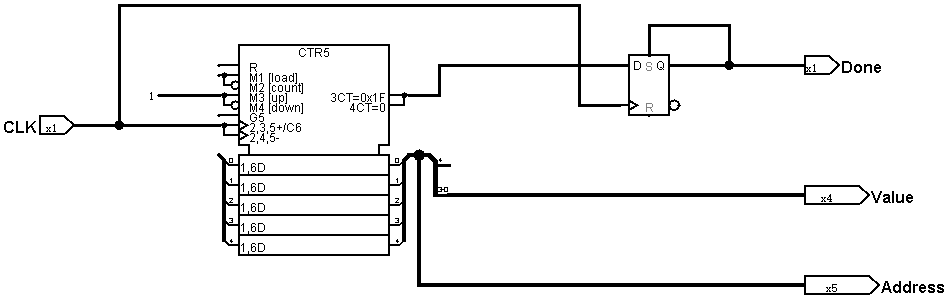
\includegraphics[width=0.3\textwidth]{memory_writer.png}
    \caption{A schematic of MemoryWriter.}
    \label{f:part1_memory_writer}
\end{figure}

\item Export the timing diagram as an image and include it in your report.

\begin{figure}[ht!]
    \centering
    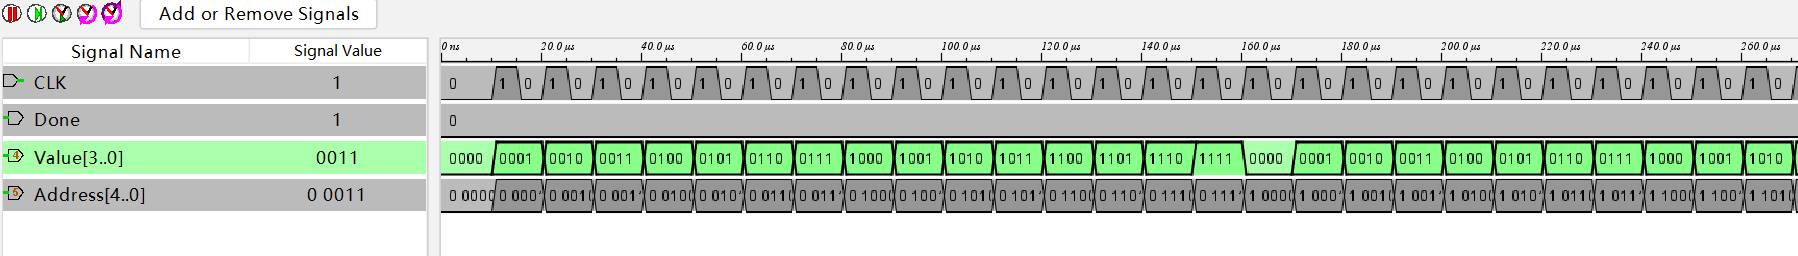
\includegraphics[width=0.65\textwidth]{lab7_part1_timing.png}
    \caption{A timing simulation of the MemoryWriter.}
    \label{f:part1_timing}
\end{figure}
\end{enumerate}

\section{Part II}

% In your report, include the schematics, timing simulations, and test vectors used in your design.
% What you choose to include will vary, but you should use earlier labs as a guide for what is likely important.
% In the end, you will need to be able to describe how your design can draw a square to your TA.
% Think carefully about which figures, tables, and Boolean equations would help in that explanation.

\begin{enumerate}
\item Export the subcircuit schematic as an image and include it in your report.

\begin{figure}[ht!]
    \centering
    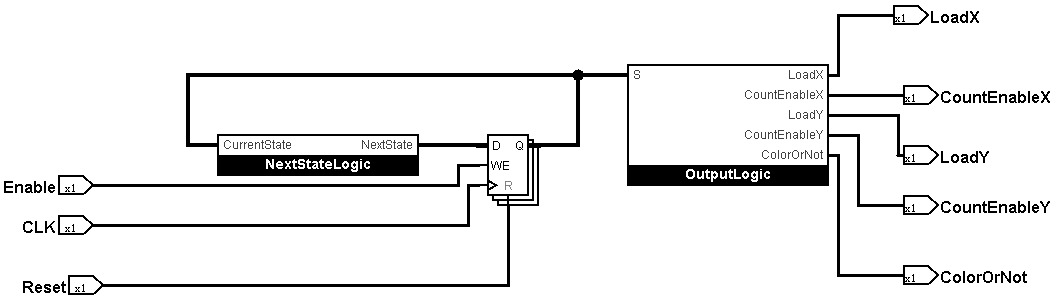
\includegraphics[width=0.3\textwidth]{ContrlUnit.png}
    \caption{A schematic of ContrlUnit.}
    \label{f:part2_ContrlUnit}
\end{figure}

\item Export the subcircuit schematic as an image and include it in your report.

\begin{figure}[ht!]
    \centering
    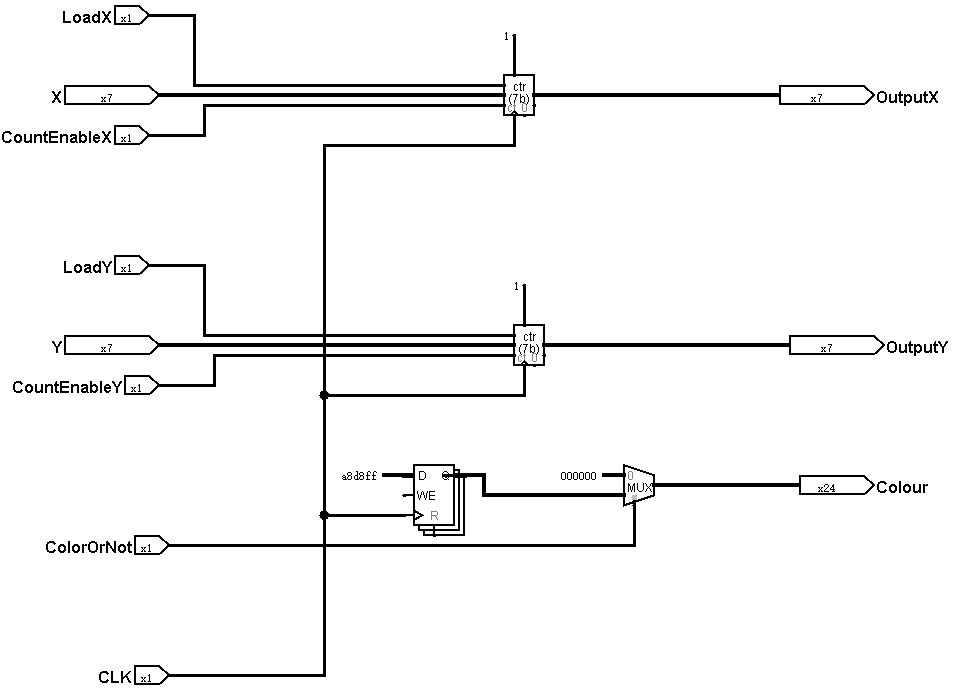
\includegraphics[width=0.3\textwidth]{DataPath.png}
    \caption{A schematic of DataPath.}
    \label{f:part2_DataPath}
\end{figure}

\item Export the subcircuit schematic as an image and include it in your report.

\begin{figure}[ht!]
    \centering
    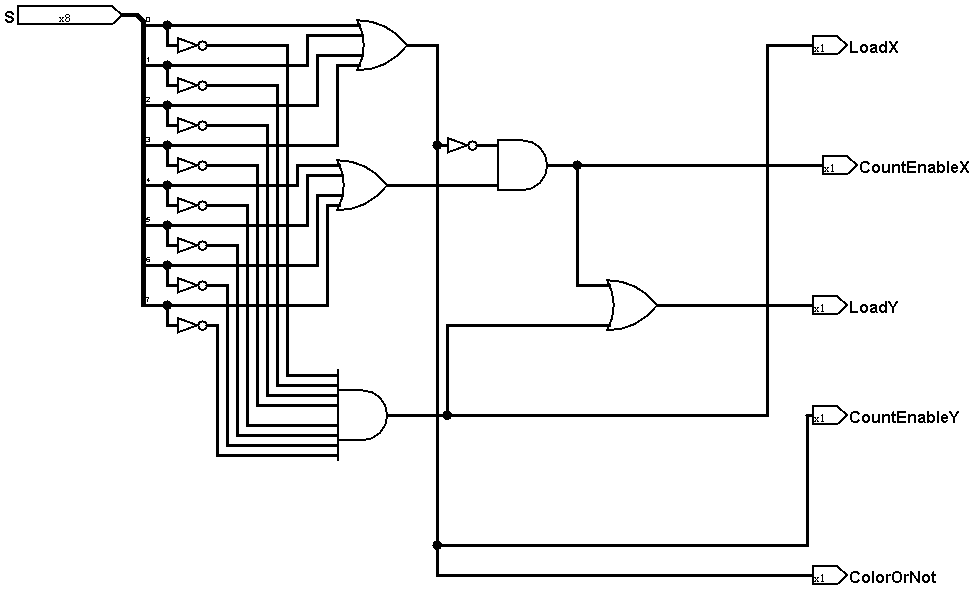
\includegraphics[width=0.3\textwidth]{OutputLogic.png}
    \caption{A schematic of OutputLogic.}
    \label{f:part2_OutputLogic}
\end{figure}

\item Export the timing simulations as an image and include it in your report.

\begin{figure}[ht!]
    \centering
    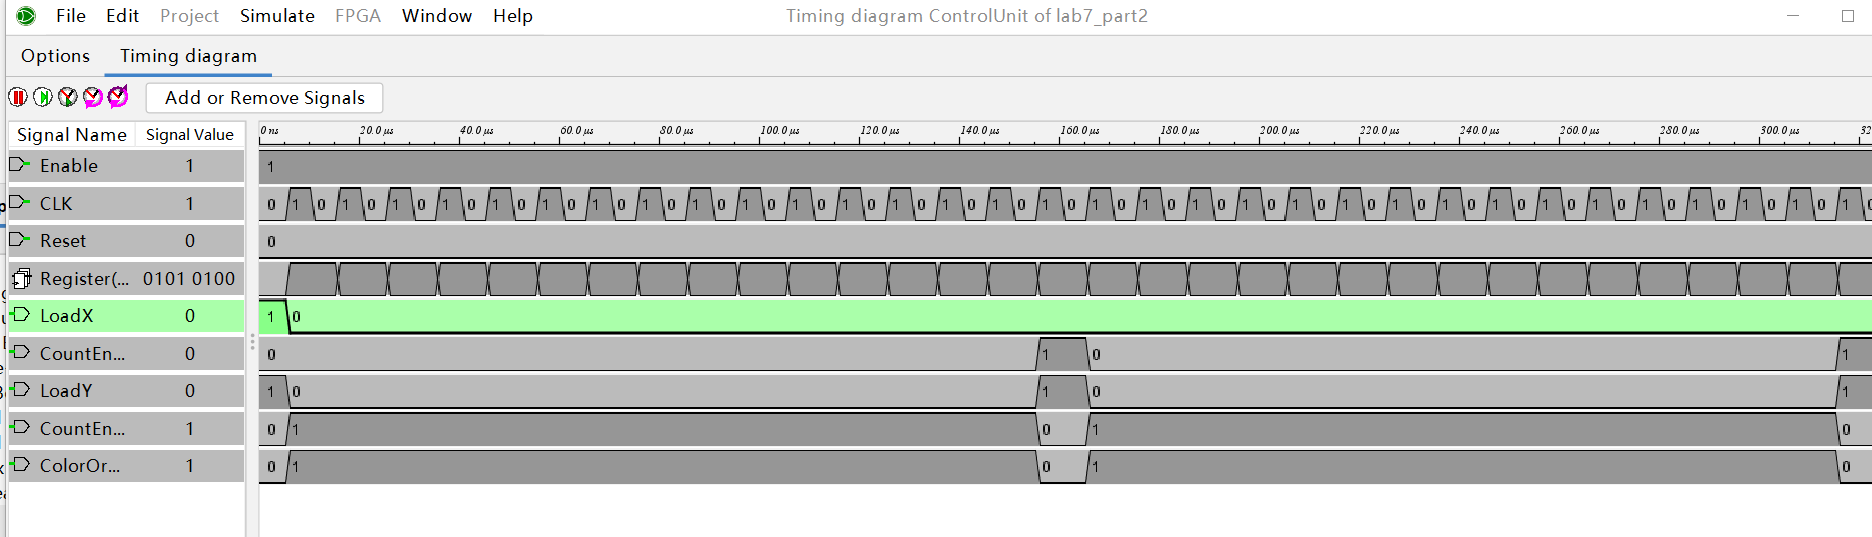
\includegraphics[width=0.3\textwidth]{timing_simulations_ContrlUnit.png}
    \caption{A schematic of timing_simulations_ContrlUnit.}
    \label{f:part2_timing_simulations_ContrlUnit}
\end{figure}

\begin{figure}[ht!]
    \centering
    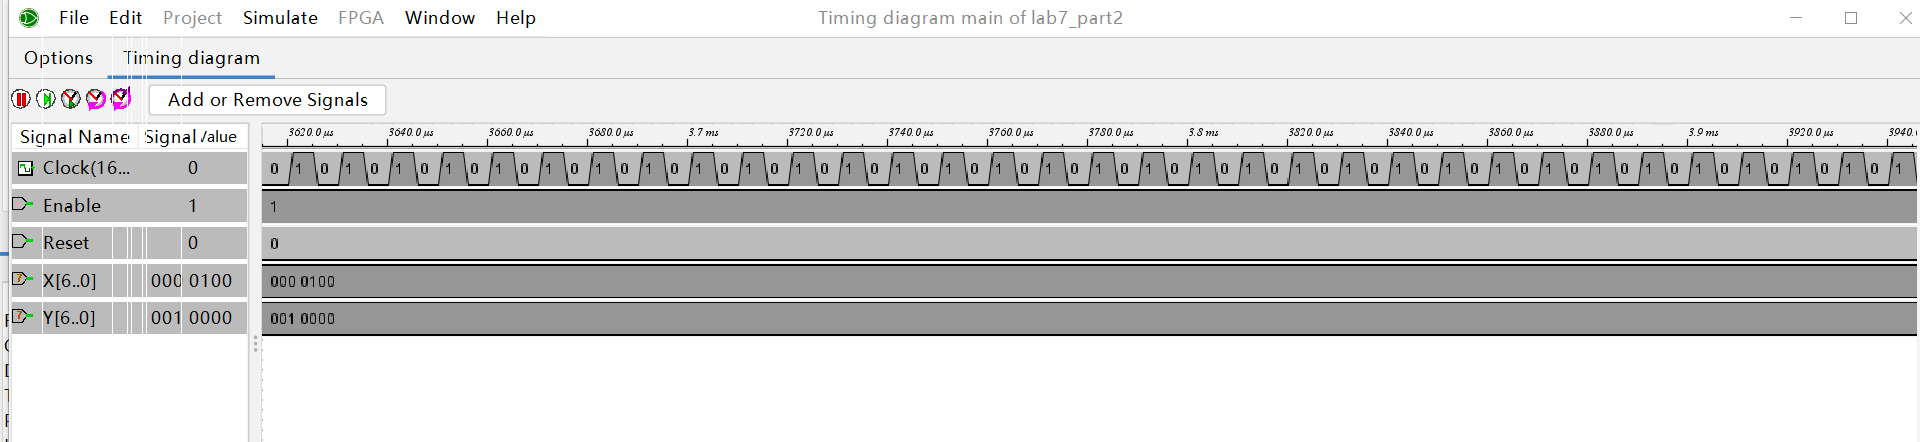
\includegraphics[width=0.3\textwidth]{timing_simulations_Main.png}
    \caption{A schematic of timing_simulations_Main.}
    \label{f:part2_timing_simulations_Main}
\end{figure}

\item Export the Test vectors as an image and include it in your report.

\begin{figure}[ht!]
    \centering
    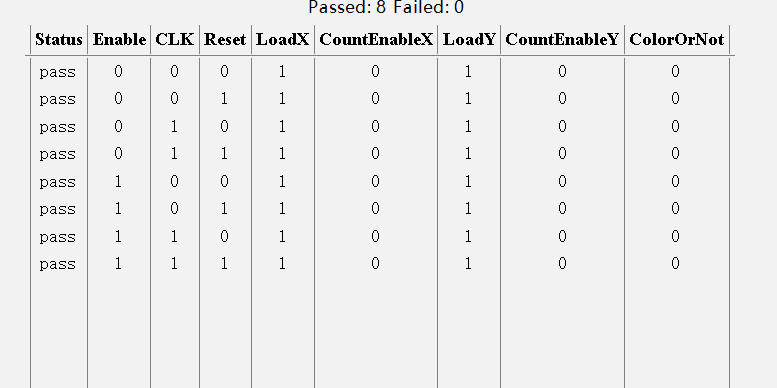
\includegraphics[width=0.3\textwidth]{Test_Vectors.png}
    \caption{A schematic of Test_Vectors of ControlUnit.}
    \label{f:part2_Test_Vectors}
\end{figure}

\end{enumerate}

\end{document}

